\documentclass{article}
\usepackage[margin=1in]{geometry}
\usepackage{pgf}
\usepackage{tikz}
\usetikzlibrary{arrows,automata}
\usepackage[latin1]{inputenc}


\newcommand\D{5}
\newcommand\scale{.8}
\newcommand\linewidthmpa{1.1pt}

\begin{document}
\begin{figure}
\center
\scalebox{\scale}{
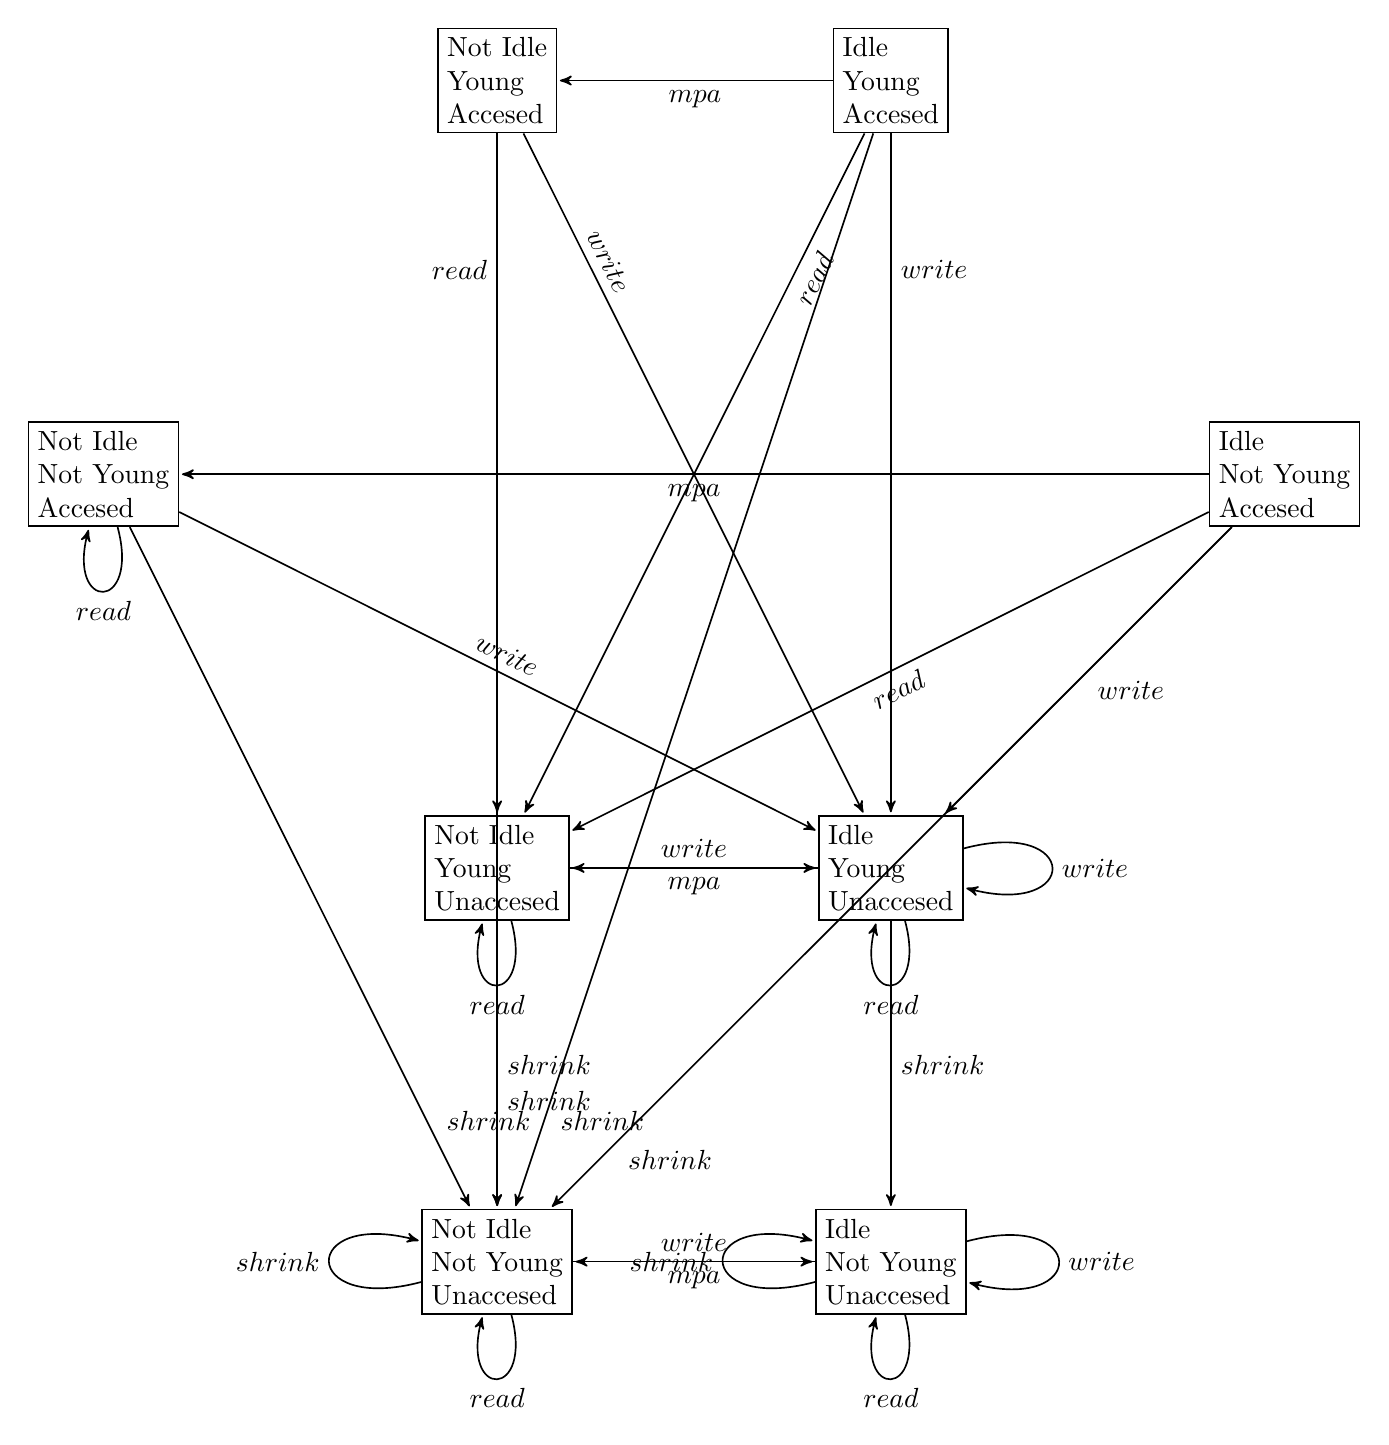
\begin{tikzpicture}[->,>=stealth',shorten >=1pt,auto,node distance=\D{}cm,
                    semithick]

  \tikzstyle{every state}=[rectangle,draw,align=left]

  \node[state] (NYA) at (0,3*\D) {Not Idle\\Young\\Accesed};    \node[state] (IYA) at (\D,3*\D) {Idle\\Young\\Accesed};

  \node[state] (NNA) at (-\D,2*\D) {Not Idle\\Not Young\\Accesed};\node[state] (INA) at (2*\D,2*\D) {Idle\\Not Young\\Accesed};

  \node[state] (NYU) at (0,\D) {Not Idle\\Young\\Unaccesed};    \node[state] (IYU) at (\D,\D) {Idle\\Young\\Unaccesed};

  \node[state] (NNU) at (0,0) {Not Idle\\Not Young\\Unaccesed}; \node[state] (INU) at (\D,0) {Idle\\Not Young\\Unaccesed};

  \path
  (NYA) edge [sloped,pos=.2] node {$write$} (IYU)
  (IYA) edge [pos=.2] node {$write$} (IYU)

  (NNA) edge [sloped]           node {$write$} (IYU)
  (INA) edge []           node {$write$} (IYU)
  (IYU) edge [loop right] node {$write$} (IYU)
  (NYU) edge [] node {$write$} (IYU)

  (NNU) edge []           node {$write$} (INU)
  (INU) edge [loop right] node {$write$} (INU)
  ;

  \path
  (NYA) edge [swap,pos=.2] node {$read$} (NYU)
  (IYA) edge [swap,sloped,pos=.2] node {$read$} (NYU)

  (NNA) edge [loop below] node {$read$} (NNA)
  (INA) edge [sloped,swap] node {$read$} (NYU)
  (IYU) edge [loop below] node {$read$} (IYU)
  (NYU) edge [loop below] node {$read$} (NYU)


  (NNU) edge [loop below] node {$read$} (NNU)
  (INU) edge [loop below] node {$read$} (INU)
  ;

  \path
  (NYA) edge [pos=.9] node {$shrink$} (NNU)
  (IYA) edge [pos=.9] node {$shrink$} (NNU)
  (INA) edge [pos=.9] node {$shrink$} (NNU)
  (NNA) edge [pos=.9] node {$shrink$} (NNU)  

  (NYU) edge [] node {$shrink$} (NNU)
  (IYU) edge [] node {$shrink$} (INU)
  (INU) edge [loop left] node {$shrink$} (INU)
  (NNU) edge [loop left] node {$shrink$} (NNU)  
  ;

  \path
  (IYA) edge [] node {$mpa$} (NYA)
  (INA) edge [] node {$mpa$} (NNA)
  (IYU) edge [] node {$mpa$} (NYU)
  (INU) edge [] node {$mpa$} (NNU)
  ;

 \end{tikzpicture}
}
\caption{Idle page tracking Automata}
\end{figure}
\end{document}
